\documentclass[letterpaper]{article}

\usepackage{fancyhdr}
\usepackage{extramarks}
\usepackage{amsmath}
\usepackage{amsthm}
\usepackage{amsfonts}
\usepackage{tikz}
\usepackage[plain]{algorithm}
\usepackage{algpseudocode}
\usepackage{amsmath}
\usepackage{verbatim}
\usepackage{graphicx}
\usepackage{epstopdf}
\usepackage{listings}
\usepackage{xcolor}

\usetikzlibrary{automata,positioning}

%
% Basic Document Settings
%

\topmargin=-0.45in
\evensidemargin=0in
\oddsidemargin=0in
\textwidth=6.5in
\textheight=9.0in
\headsep=0.25in

\linespread{1.1}

\pagestyle{fancy}
\lhead{\hmwkAuthorName}
%\chead{\hmwkClass\ (\hmwkClassInstructor): \hmwkTitle}
\rhead{\hmwkAuthorUNI}
\lfoot{\lastxmark}
\cfoot{\thepage}

\renewcommand\headrulewidth{0.4pt}
\renewcommand\footrulewidth{0.4pt}

\setlength\parindent{0pt}

%
% Create Problem Sections
%

\newcommand{\enterProblemHeader}[1]{
    %\nobreak\extramarks{}{Problem \arabic{#1} continued on next page\ldots}\nobreak{}
    %\nobreak\extramarks{Problem \arabic{#1} (continued)}{Problem \arabic{#1} continued on next page\ldots}\nobreak{}
}

\newcommand{\exitProblemHeader}[1]{
    %\nobreak\extramarks{Problem \arabic{#1} (continued)}{Problem \arabic{#1} continued on next page\ldots}\nobreak{}
    \stepcounter{#1}
    %\nobreak\extramarks{Problem \arabic{#1}}{}\nobreak{}
}

\setcounter{secnumdepth}{0}
\newcounter{partCounter}
\newcounter{homeworkProblemCounter}
\setcounter{homeworkProblemCounter}{1}
\nobreak\extramarks{Problem \arabic{homeworkProblemCounter}}{}\nobreak{}

\newenvironment{homeworkProblem}{
    \section{Problem \arabic{homeworkProblemCounter}}
    \setcounter{partCounter}{0}
    \enterProblemHeader{homeworkProblemCounter}
}{
    \exitProblemHeader{homeworkProblemCounter}
}

%
% Homework Details
%   - Title
%   - Due date
%   - Class
%   - Section/Time
%   - Instructor
%   - Author
%

\newcommand{\hmwkTitle}{Homework\ \#1}
\newcommand{\hmwkDueDate}{September 18, 2017}
\newcommand{\hmwkClass}{LINEAR REGRESSION MODELS}
%\newcommand{\hmwkClassTime}{Section 005}
\newcommand{\hmwkClassInstructor}{Professor Jingchen Liu}
\newcommand{\hmwkAuthorName}{Fan Yang}
\newcommand{\hmwkAuthorUNI}{UNI: fy2232}

%
% Title Page
%

\title{
    \vspace{2in}
    \textmd{\textbf{\hmwkClass:\ \hmwkTitle}}\\
    \normalsize\vspace{0.1in}\small{Due\ on\ \hmwkDueDate}\\
    \vspace{0.1in}\large{\textit{\hmwkClassInstructor}}
    \vspace{3in}
}

\author{\textbf{\hmwkAuthorName}\\
    \text{\hmwkAuthorUNI}}
\date{}

\renewcommand{\part}[1]{\textbf{\large Part \Alph{partCounter}}\stepcounter{partCounter}\\}

%
% Various Helper Commands
%

% Useful for algorithms
\newcommand{\alg}[1]{\textsc{\bfseries \footnotesize #1}}

% For derivatives
\newcommand{\deriv}[1]{\frac{\mathrm{d}}{\mathrm{d}x} (#1)}

% For partial derivatives
\newcommand{\pderiv}[2]{\frac{\partial}{\partial #1} (#2)}

% Integral dx
\newcommand{\dx}{\mathrm{d}x}

% Alias for the Solution section header
\newcommand{\solution}{\textbf{\large Solution}}

% Probability commands: Expectation, Variance, Covariance, Bias
\newcommand{\E}{\mathrm{E}}
\newcommand{\Var}{\mathrm{Var}}
\newcommand{\Cov}{\mathrm{Cov}}
\newcommand{\Bias}{\mathrm{Bias}}

\begin{document}

\maketitle
\setcounter{page}{0}
\thispagestyle{empty}

\pagebreak

\begin{homeworkProblem}     %1

    \textbf{a.}
    \begin{verbatim}
    da = read.table("CH01PR19.txt")
    lm.pr19<-lm(da$V1~da$V2)
    summary(lm.pr19)   \end{verbatim}
    ~~~~~~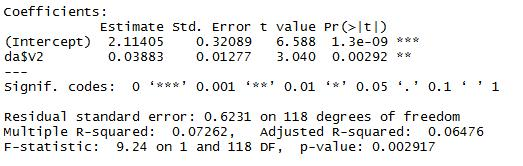
\includegraphics[width=4in]{reg_hw1_pic12.jpg}
    \[
        \begin{split}
            &therefore~\widehat{y}=2.44105+0.03883x
            \\
        \end{split}
    \]

    \textbf{b.}
    ~~~~~~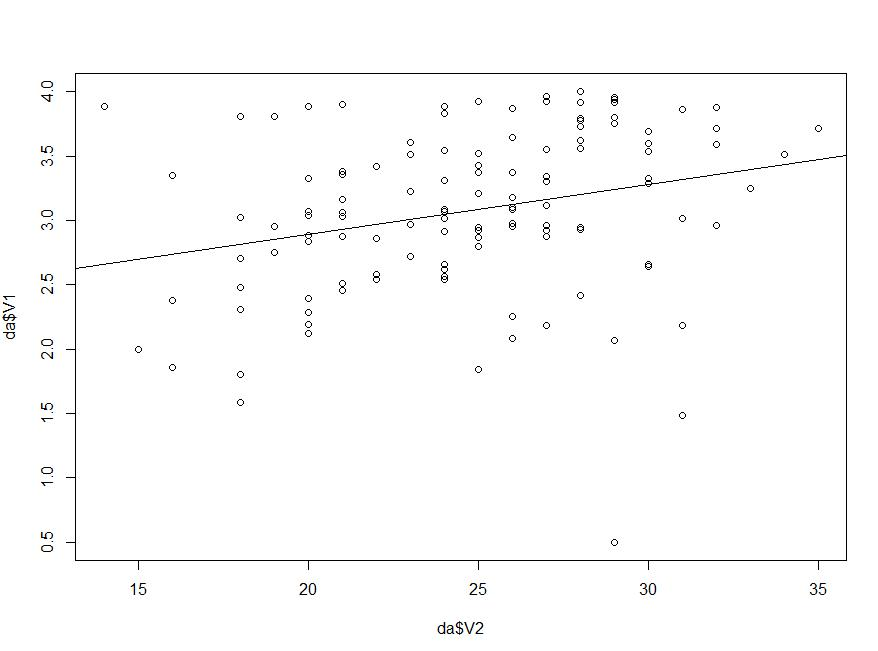
\includegraphics[height=3.5in]{reg_hw1_pic13.jpg}

    \[
        \begin{split}
            &\text{when a x is fixed, there could be some different possible y. so the relation between x and y could.}\\
            &\text{not be linear. We can draw conclusion from the plot above that the function does not fit the data.}
        \end{split}
    \]
    \textbf{c.}

    \[
        \begin{split}
        &\text{When X=30, we apply the function in (a)}\\
        &\widehat{y}=\beta_0+\beta_1*x\\
        &=2.11405+0.03883*30=3.27895
        \end{split}
    \]

    \textbf{d.}

    \[
        \begin{split}
            \Delta y=&y_1-y_2=(2.11405+0.03883*x)-(2.11405+0.03883*(x+1))=0.03883
        \end{split}
    \]

\end{homeworkProblem}

\begin{homeworkProblem}%2

    \[
        \begin{split}
            &\text{When $\beta_0$ is 0,we know that the regression model only determines by $\beta_1$,and the function line goes}\\
            &\text{through origin point and is a linear line which only depends on the slope.}\\
        \end{split}
    \]

\end{homeworkProblem}

\begin{homeworkProblem}     %3

    \[
        \begin{split}
            &\text{When $\beta_1$ is 0,the response variable is a constant and no longer related to explanatory variable.}\\
            &\text{And $Y_i$ always equal to $\beta_0$. The regression now becomes horizontal.}\\
        \end{split}
    \]

\end{homeworkProblem}

\begin{homeworkProblem}     %4
    \[
        \begin{split}
    &\text{the goal of least squares estimator is to minimize}\sum_i^n (y_i-\beta_0)^2\\
    &\sum_i^n (y_i-\beta_0)^2=\sum_i^n (y_i-\overline{y}+\overline{y}-\beta_0)^2
    =\sum_i^n (y_i-\overline{y})^2-2\sum_i^n (y_i-\overline{y})(\overline{y}-\beta_0)+\sum_i^n (\overline{y}-\beta_0)^2\\
    &=\sum_i^n (y_i-\overline{y})^2+\sum_i^n (\overline{y}-\beta_0)^2\\
    &\text{in order to minimize the above statement, $\beta_0$ should be equal to $\overline{y}$.}\\
    &\text{Therefore,least squares estimator of $\beta_0$ is }\widehat{\beta_0}=\overline{y}\\
        \end{split}
    \]
\end{homeworkProblem}

\begin{homeworkProblem}     %5

    \[
        \begin{split}
        E(\widehat{\beta}_0)&=E(\overline{y})=E(\frac{1}{n}\sum y_i)\\
        &=\frac{1}{n}E(\sum y_i)=\frac{1}{n}\sum E( y_i)=\frac{1}{n}\sum E(\beta_0)
        =\frac{1}{n}*n*\beta_0\\
        &=\beta_0\\
        \text{so that $\widehat{\beta}_0$ is unbiased}\\
        \end{split}
    \]


\end{homeworkProblem}

\begin{homeworkProblem}     %6

    \textbf{a.}
    \[
        \begin{split}
        &\text{We use the following conclusion without proof}\\
        &\widehat{\beta}_1=\frac{\sum(x_i-\overline{x})(y_i-\overline{y})}{(\sum x_i-\overline{x})^2}\\
        &\widehat{\beta}_0=\overline{y}-\widehat{\beta}_1 \overline{x}\\
        &\overline{x}=10\\
        \\
        &\text{denote $\overline{Y}$ as the mean of the 6 observations( also the mean of 3 means of observations)}\\
        &\text{1) in the 3 points regression}\\
        &\widehat{\beta}_1^1=\frac{(5-10)(\overline{Y}_1-\overline{Y})+(10-10)(\overline{Y}_2-\overline{Y})+(15-10)(\overline{Y}_3-\overline{Y})}
        {(5-10)^2+(10-10)^2+(15-10)^2}\\
        &=\frac{-5(\overline{Y}_1-\overline{Y})+5(\overline{Y}_3-\overline{Y})}{50}
        =\frac{\overline{Y}_3-\overline{Y}_1}{10}\\
        \\
        &\text{2) in the 6 points regression}\\
        &\widehat{\beta}_1^2=\\
        &\frac{(5-10)[(Y_{11}-\overline{Y})+(Y_{12}-\overline{Y})]
        +(10-10)[(Y_{21}-\overline{Y})+(Y_{22}-\overline{Y})]
        +(15-10)[(Y_{32}-\overline{Y})+(Y_{33}-\overline{Y})]}
        {2*(5-10)^2+2*(10-10)^2+2*(15-10)^2}\\
        &=\frac{-5(Y_{11}-\overline{Y}+Y_{12}-\overline{Y})+5(Y_{31}-\overline{Y}+Y_{32}-\overline{Y})}{100}\\
        &=\frac{-5(2\overline{Y}_1-2\overline{Y})+5(2\overline{Y}_3-2\overline{Y})}{100}\\
        &=\frac{\overline{Y}_3-\overline{Y}_1}{10}\\
        &=\widehat{\beta}_1^1\\
        \\
        &\text{that's to say, the $\widehat{\beta}_1$ in two models are identical}\\
        &\text{Besides, $\overline{x}$ and $\overline{y}$ are same in two models.}\\
        &\text{according to $\widehat{\beta}_0=\overline{y}-\widehat{\beta}_1 \overline{x}$ we know $\widehat{\beta}_0$ are same.}\\
        &\text{therefore, the two regression lines are identical.}
        \end{split}
    \]
%\newpage
    \textbf{b.}
    \[
        \begin{split}
        &\widehat{\sigma}^2=\frac{\sum(y_i-\widehat{y}_i)^2}{n-2}=\frac{\sum(y_i-\widehat{\beta}_0-\widehat{\beta}_1x_i)^2}{n-2}\\
        &=(\overline{Y}_1-\widehat{\beta}_0-\widehat{\beta}_1X_1)^2+(\overline{Y}_2-\widehat{\beta}_0-\widehat{\beta}_1X_2)^2+(\overline{Y}_3-\widehat{\beta}_0-\widehat{\beta}_1X_3)^2\\
        &=(\overline{Y}_1-\widehat{\beta}_0-5\widehat{\beta}_1)^2+(\overline{Y}_2-\widehat{\beta}_0-10\widehat{\beta}_1)^2+(\overline{Y}_3-\widehat{\beta}_0-15\widehat{\beta}_1)^2\\
        &\text{from a we know }\widehat{\beta}_1=\frac{\overline{Y}_3-\overline{Y}_1}{10}~\text{and }
         \widehat{\beta}_0=\overline{Y}-\widehat{\beta}_1 \overline{X}\\
        &\text{then }\widehat{\sigma}^2=(\overline{Y}_1-\overline{Y})^2+(\frac{(\overline{Y}_1+4\overline{Y}_2-5\overline{Y}_3}{6})^2+(\overline{Y}_1-\overline{Y})^2\\
        &=2(\frac{2\overline{Y}_1-\overline{Y}_2-\overline{Y}_3}{3})^2+(\frac{(\overline{Y}_1+4\overline{Y}_2-5\overline{Y}_3}{6})^2\\
        &\text{Thus, we only need to apply $\overline{Y}_1~\overline{Y}_2~\overline{Y}_3$ to above equation, then we will get the estimator of $\sigma^2$ without}\\
        &\text{fitting a regression line}
        \end{split}
    \]

\end{homeworkProblem}


\begin{homeworkProblem}     %7

    \textbf{a.}

    \[
        \begin{split}
        &\text{We use the following conclusion without proof}\\
        &\widehat{\beta}_1=\frac{\sum(x_i-\overline{x})(y_i-\overline{y})}{(\sum x_i-\overline{x})^2}\\
        &\widehat{\beta}_0=\overline{y}-\widehat{\beta}_1 \overline{x}\\
        &\text{since we know that $\beta_0=0$ }\\
        &\text{now our goal is to minimize}\sum_i^n(y_i-\beta_1x_i)^2\\
        &\sum_i^n(y_i-\beta_1x_i)^2=\sum_i^n[y_i-\overline{y}+\beta_1\overline{x}-\beta_1x_i]^2\\
        &=\sum_i^n(y_i-\overline{y})^2+2\sum_i^n(y_i-\overline{y})(\beta_1\overline{x}-\beta_1x_i)
        +\sum_i^n(\beta_1\overline{x}-\beta_1x_i)^2\\
        &=\sum_i^n(y_i-\overline{y})^2+\sum_i^n(\beta_1\overline{x}-\beta_1x_i)^2\\
        &=\sum_i^n(y_i-\overline{y})^2+\beta_1^2\sum_i^n(\overline{x}-x_i)^2\\
        &=\sum_i^n(x_i-\overline{x})^2\left(\beta_1-\frac{\sum(x_i-\overline{x})(y_i-\overline{y})}{\sum(x_i-\overline{x})^2}\right)^2
        +\sum_i^n(y_i-\overline{y})^2-\frac{(\sum(x_i-\overline{x})(y_i-\overline{y}))^2}{\sum(x_i-\overline{x})^2}\\
        &\Rightarrow \widehat{\beta}_1=\frac{\sum(x_i-\overline{x})(y_i-\overline{y})}{\sum(x_i-\overline{x})^2}\\
        \end{split}
    \]

    \textbf{b.}

    \[
        \begin{split}
        &\varepsilon_i\sim N(0,\sigma^2),pdf=\frac{1}{\sigma \sqrt{2\pi}}exp\left(-\frac{x^2}{2\sigma^2}\right)\\
        &L(\beta_1,\sigma)=\prod \limits_{i}^{n} \frac{1}{\sigma \sqrt{2\pi}}exp\left(-\frac{(Y_i-\beta_1X_i)^2}{2\sigma^2}\right)\\
        &=\frac{1}{(\sigma \sqrt{2\pi})^n} exp\left(-\frac{\sum\limits_{i}^{n} (Y_i-\beta_1X_i)^2}{2\sigma^2}\right)\\
        &\text{in order to maximize $L(\beta_1,\sigma)$, we simply only need to minimize $\sum\limits_{i}^{n} (Y_i-\beta_1X_i)^2$}\\
        &\text{now it becomes the same problem as least square estimate, therefore the two estimator of $\beta_1$ are}\\
        &\text{identical.}\\
        &\widehat{\beta}_1=\frac{\sum\limits _i^n(x_i-\overline{x})(y_i-\overline{y})}{\sum\limits _i^n(x_i-\overline{x})^2}\\
        \end{split}
    \]

    \textbf{c.}

    \[
        \begin{split}
        &\widehat{\beta}_1=\frac{\sum\limits _i^n(x_i-\overline{x})(y_i-\overline{y})}{\sum\limits _i^n(x_i-\overline{x})^2}\\
        &E(\widehat{\beta}_1)=E(\frac{\sum\limits _i^n(x_i-\overline{x})(y_i-\overline{y})}{\sum\limits _i^n(x_i-\overline{x})^2})
        =\frac{\sum\limits _i^n(x_i-\overline{x})E(y_i-\overline{y})}{\sum\limits _i^n(x_i-\overline{x})^2}
        =\frac{\sum\limits _i^n(x_i-\overline{x})(E(y_i)-\overline{y})}{\sum\limits _i^n(x_i-\overline{x})^2}\\
        &\text{because }E(y_i)=\beta_1x_i~~and~~ \overline{y}=\beta_1x_i~;\\
        &E(\widehat{\beta}_1)=\frac{\sum\limits _i^n(x_i-\overline{x})(\beta_1x_i-\overline{y})}{\sum\limits _i^n(x_i-\overline{x})^2}
        =\frac{\sum\limits _i^n(x_i-\overline{x})(\beta_1x_i-\beta_1\overline{x})}{\sum\limits _i^n(x_i-\overline{x})^2}
        =\frac{\beta_1\sum\limits _i^n(x_i-\overline{x})(x_i-\overline{x})}{\sum\limits _i^n(x_i-\overline{x})^2}\\
        &=\beta_1\\
        &\text{therefore $\widehat{\beta}_1$ is unbiased.}\\
        \end{split}
    \]

\end{homeworkProblem}

\begin{homeworkProblem}     %8
    \[
    \begin{split}
    &\text{Firstly we get the observation data. Let d be the raw data. Y is number of active physicians }\\
        \text{and X}&\text{ is the combination of the three predictor variables.}\\
    \end{split}
    \]
    \begin{verbatim}
    Y <- d$`Number of active physicians`
    X <- cbind(d$`Total population`, d$`Number of hospital beds`, d$`Total personal income`)
    \end{verbatim}

    \textbf{(1)}
    \[
        \begin{split}
        &\text{a. Regress the number of active physicians on}\textbf{ total population.}\\
        \end{split}
    \]
    \begin{verbatim}
        lm.cdi1 <- lm(Y~X[,1])
        summary(lm.cdi1)
    \end{verbatim}
    \[~~~~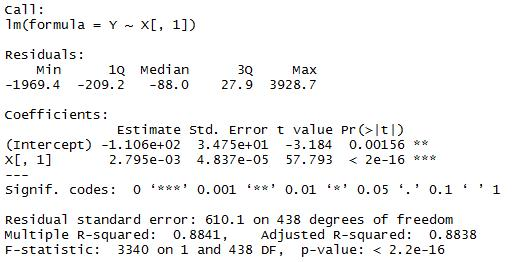
\includegraphics[width=4.3in,height=2in]{reg_hw1_pic2.jpg}\\\]
    \[
        ~~~~\text{we get the regression function }Y=-110.6+2.795\times10^{-3}X
    \]

    \[
        \begin{split}
        &\text{b. Regress the number of active physicians on}\textbf{ number of hospital beds.}\\
        \end{split}
    \]
    \begin{verbatim}
        lm.cdi2 <- lm(Y~X[,2])
        summary(lm.cdi2)
    \end{verbatim}
    \[~~~~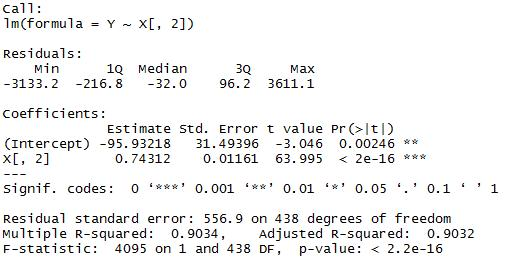
\includegraphics[width=4.3in,height=2in]{reg_hw1_pic3.jpg}\\\]
    \[
        ~~~~\text{we get the regression function }Y=-95.932+0.743X
    \]
    \[
        \begin{split}
        &\text{c. Regress the number of active physicians on}\textbf{ total personal income.}\\
        \end{split}
    \]
    \begin{verbatim}
        lm.cdi3 <- lm(Y~X[,3])
        summary(lm.cdi3)
    \end{verbatim}
    \[~~~~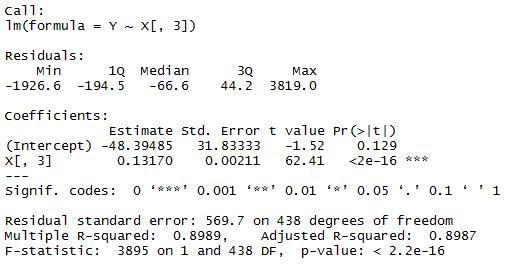
\includegraphics[width=4.3in,height=2in]{reg_hw1_pic4.jpg}\\\]
    \[
        ~~~~\text{we get the regression function }Y=-48.395+0.132X
    \]

    \textbf{(2)}
    \[~~~~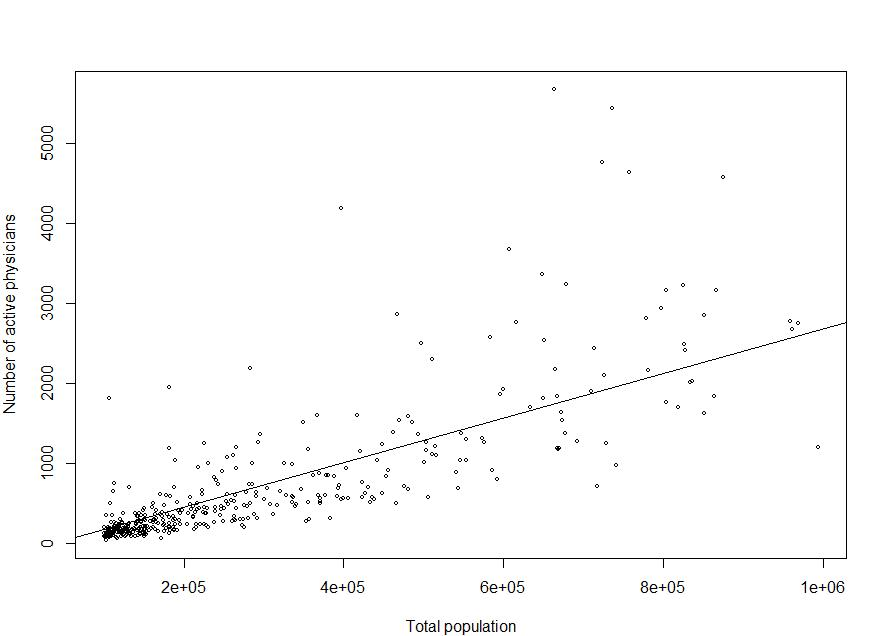
\includegraphics[width=5.5in]{reg_hw1_pic5.jpg}\\\]
    \[~~~~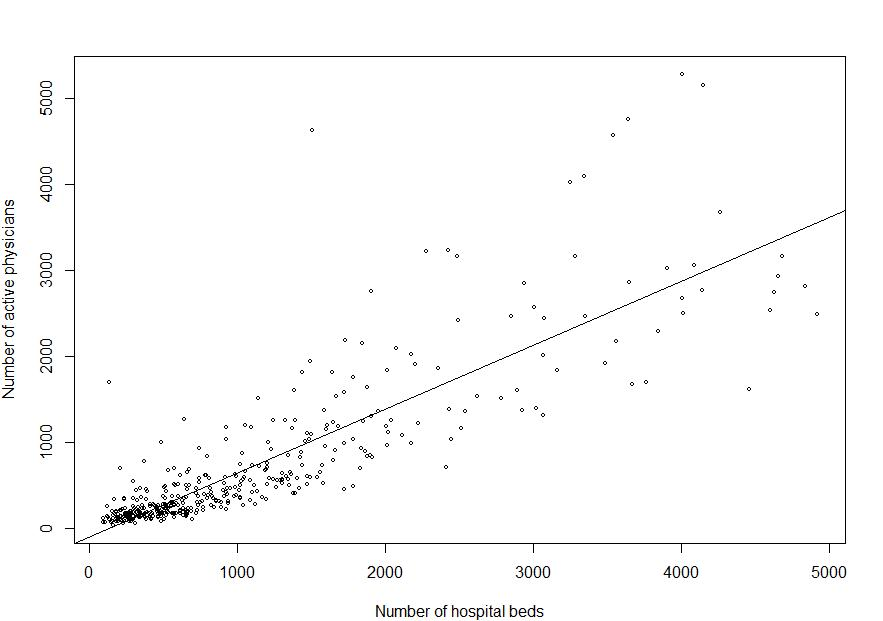
\includegraphics[width=5.5in]{reg_hw1_pic6.jpg}\\\]
    \[~~~~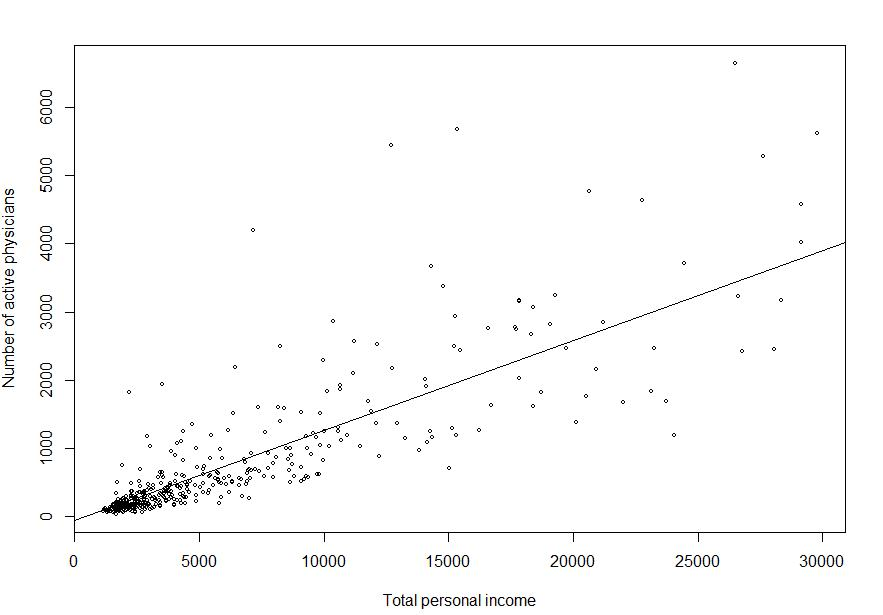
\includegraphics[width=5.5in]{reg_hw1_pic7.jpg}\\\]
        \text{ from 3 plots above, we find that simple linear regression line somehow depicts the relation between X}\\
        \text{and Y. Besides the P-values in each model are less than 0.001, so the regression lines seem to be a good}\\
        \text{fit for each of the predictor variables}\\
    \textbf{(3)}
    \begin{verbatim}
        MSE1 <- sum(lm.cdi1$residuals^2)/(440-2)
        [1] 372203.5
    \end{verbatim}

    \begin{verbatim}
        MSE2 <- sum(lm.cdi2$residuals^2)/(440-2)
        [1] 310191.9
    \end{verbatim}
    \begin{verbatim}
        MSE3 <- sum(lm.cdi3$residuals^2)/(440-2)
        [1] 324539.4
    \end{verbatim}
    \text{ from the results above, we can conclude that the variable}\textbf{ number of hospital beds}\text{ leads to the smallest}
    \text{variability.}
\end{homeworkProblem}

\begin{homeworkProblem}     %9
    \text{Let Yi be per capita income and Xi be the percentage of individuals having }
    \text{bachelor's degree in $i^{th}$ region.}
    \begin{verbatim}
    Y1<-d$`Per capita income`[d$`Geographic region`==1]
    X1<-d$`Percent bachelor's degrees`[d$`Geographic region`==1]
    Y2<-d$`Per capita income`[d$`Geographic region`==2]
    X2<-d$`Percent bachelor's degrees`[d$`Geographic region`==2]
    Y3<-d$`Per capita income`[d$`Geographic region`==3]
    X3<-d$`Percent bachelor's degrees`[d$`Geographic region`==3]
    Y4<-d$`Per capita income`[d$`Geographic region`==4]
    X4<-d$`Percent bachelor's degrees`[d$`Geographic region`==4]
    \end{verbatim}

    \textbf{(1)}
    \[
        \begin{split}
        &\text{ Regress the }\textbf{ per capita income}\text{ on}\textbf{ total population}\text{ for the}\textbf{ first}\text{ region}\\
        \end{split}
    \]
    \begin{verbatim}
        lm.cdi1<-lm(Y1~X1)
        summary(lm.cdi1)
    \end{verbatim}
    \[~~~~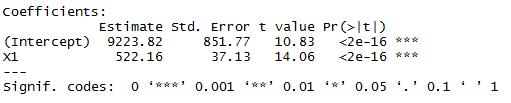
\includegraphics[width=4in]{reg_hw1_pic8.jpg}\\\]
    \[
        ~~~~\text{we get the regression function }Y=9223.82+522.16X
    \]

    \[
        \begin{split}
        &\text{ Regress the }\textbf{ per capita income}\text{ on}\textbf{ total population}\text{ for the}\textbf{ second}\text{ region}\\
        \end{split}
    \]
    \begin{verbatim}
        lm.cdi2<-lm(Y2~X2)
        summary(lm.cdi2)
    \end{verbatim}
    \[~~~~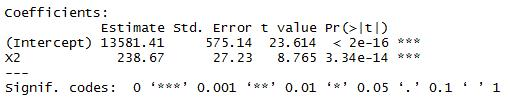
\includegraphics[width=4in]{reg_hw1_pic9.jpg}\\\]
    \[
        ~~~~\text{we get the regression function }Y=13581.41+238.67X
    \]

    \[
        \begin{split}
        &\text{ Regress the }\textbf{ per capita income}\text{ on}\textbf{ total population}\text{ for the}\textbf{ third}\text{ region}\\
        \end{split}
    \]
    \begin{verbatim}
        lm.cdi3<-lm(Y3~X3)
        summary(lm.cdi3)
    \end{verbatim}
    \[~~~~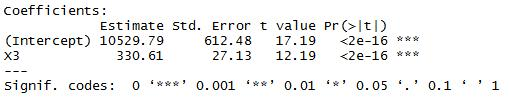
\includegraphics[width=4in]{reg_hw1_pic10.jpg}\\\]
    \[
        ~~~~\text{we get the regression function }Y=10529.79+330.61X
    \]

    \[
        \begin{split}
        &\text{ Regress the }\textbf{ per capita income}\text{ on}\textbf{ total population}\text{ for the}\textbf{ forth}\text{ region}\\
        \end{split}
    \]
    \begin{verbatim}
        lm.cdi4<-lm(Y4~X4)
        summary(lm.cdi4)
    \end{verbatim}
    \[~~~~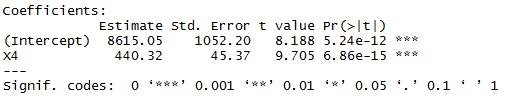
\includegraphics[width=4in]{reg_hw1_pic11.jpg}\\\]
    \[
        ~~~~\text{we get the regression function }Y=8615.05+440.32X
    \]

    \textbf{(2)}
    \[
        \begin{split}
        &\text{Let R1 = 1 if in region 1; otherwise 0; Let R2 = 1 if in region 2; otherwise 0;}\\
        &\text{Let R3 = 1 if in region 3; otherwise 0;}\\
        &\text{Let X,Y be the }\textbf{per capita income}\text{ and}\textbf{ total population }\text{,respectively.}\\
        &\text{Then we apply full model }\\
        &Y=\beta_0+\beta_1X+\beta_2R1X+\beta_3R2X+\beta_3R3X+\varepsilon\\
        \end{split}
    \]
        \begin{verbatim}
        > lm.full <- lm(Y~X+R1*X+R2*X+R3*X)
        \end{verbatim}
    \[
        \begin{split}
        &\text{If there is no region effect, then the reduced model is}\\
        &Y=\beta_0+\beta_1X+\varepsilon\\
        \end{split}
    \]
    \begin{verbatim}
        > lm.reduce <- lm(Y~X)
    \end{verbatim}
        For the full model,we have\\
        \begin{verbatim}
        > sum(lm.full$residuals^2)
        [1] 2945664166
        > lm.full$df.residual
        [1] 432
        \end{verbatim}
        \[~~~~~~~~~~~~SSE=3496250017~~~~~~DF=432\]
        For the reduced model,we have
        \begin{verbatim}
        > sum(lm.reduce$residuals^2)
        [1] 3735858256
        > lm.reduce$df.residual
        [1] 438
        \end{verbatim}
        \[~~~~~~~~~~~~SSE=3735858256~~~~~~DF=438\]
        Thus\[F^*=\frac{(3735858256-2945664166)/(438-432)}{2945664166/432}\]
        \[~~~~=19.31448>F_{95\%}(6,432)=2.12\]\\
        \textbf{Therefore, region matters, which means different region have different regression functions.}\\

    \textbf{(3)}
    \begin{verbatim}
        MSE1 <- sum(lm.cdi1$residuals^2)/lm.cdi1$df.residual
        [1] 7335008
    \end{verbatim}

    \begin{verbatim}
        MSE2 <- sum(lm.cdi2$residuals^2)/lm.cdi2$df.residual
        [1] 4411341
    \end{verbatim}
    \begin{verbatim}
        MSE3 <- sum(lm.cdi3$residuals^2)/lm.cdi3$df.residual
        [1] 7474349
    \end{verbatim}
    \begin{verbatim}
        MSE4 <- sum(lm.cdi4$residuals^2)/lm.cdi4$df.residual
        [1] 8214318
    \end{verbatim}
    \text{ from the results above, we can conclude that the variable around the fitted regression line differs }\\
    \text{from each other. But the variable for region \#1 and \#3 are approximately the same.}
\end{homeworkProblem}


\end{document}
